\documentclass{article}


% if you need to pass options to natbib, use, e.g.:
%     \PassOptionsToPackage{numbers, compress}{natbib}
% before loading neurips_2023


% ready for submission
\usepackage[final]{neurips_2023}


% to compile a preprint version, e.g., for submission to arXiv, add add the
% [preprint] option:
%     \usepackage[preprint]{neurips_2023}


% to compile a camera-ready version, add the [final] option, e.g.:
%     \usepackage[final]{neurips_2023}


% to avoid loading the natbib package, add option nonatbib:
%    \usepackage[nonatbib]{neurips_2023}


\usepackage[utf8]{inputenc} % allow utf-8 input
\usepackage[T1]{fontenc}    % use 8-bit T1 fonts
\usepackage{hyperref}       % hyperlinks
\usepackage{url}            % simple URL typesetting
\usepackage{booktabs}       % professional-quality tables
\usepackage{amsfonts}       % blackboard math symbols
\usepackage{amsmath}
\usepackage{nicefrac}       % compact symbols for 1/2, etc.
\usepackage{microtype}      % microtypography
\usepackage{xcolor}         % colors
\usepackage{graphicx}       % images
\usepackage{float}          % use the [H] option for figure placement


\title{Project Proposal: Transformer-based Model for Mathematical Problem Solving}


% The \author macro works with any number of authors. There are two commands
% used to separate the names and addresses of multiple authors: \And and \AND.
%
% Using \And between authors leaves it to LaTeX to determine where to break the
% lines. Using \AND forces a line break at that point. So, if LaTeX puts 3 of 4
% authors names on the first line, and the last on the second line, try using
% \AND instead of \And before the third author name.


\author{%
    Chau Nguyen \\
    \texttt{chauminh.nguyen@mail.utoronto.ca} \\
    \and
    Gabriel You \\
    \texttt{gabriel.you@mail.utoronto.ca} \\
    \and
    Takia Talha \\
    \texttt{takia.talha@mail.utoronto.ca} \\
    \and
    Taha Siddiqi \\
    \texttt{taha.siddiqi@mail.utoronto.ca} \\
    \\
    Department of Mathematical \& Computational Sciences \\
    University of Toronto Mississauga
}
\begin{document}

\maketitle


\begin{abstract}
%   The abstract paragraph should be indented \nicefrac{1}{2}~inch (3~picas) on
%   both the left- and right-hand margins. Use 10~point type, with a vertical
%   spacing (leading) of 11~points.  The word \textbf{Abstract} must be centered,
%   bold, and in point size 12. Two line spaces precede the abstract. The abstract
%   must be limited to one paragraph.

%   A short description of your goals, task, model, and (for
% the final report) results. The abstract should make the
% motivations and the scope of your project clear so that
% readers can decide whether they are interested in
% reading your work.
  Mathematical problem solving often requires both symbolic manipulation and natural language understanding. In this paper, we propose a hybrid, lightweight, and open-source model that combines reason-based mathematics with deep learning to solve mathematical problems expressed in natural language or LaTeX format. Our approach integrates several powerful components:\texttt{MathBERT} for tokenizing and encoding both natural language and symbolic math content, and a T5 architecture featuring an encoder-decoder structure to generate a LATEX formatted answer to math word problems. This architecture allows the model to handle complex mathematical reasoning tasks, from simple algebraic equations to advanced calculus, while providing accurate and interpretable solutions. We demonstrate that our  model leverages the strengths of neural approaches to deliver a more robust solution for automated math problem-solving. Our code and final report is available for review at our \href{https://github.com/chloe-nguyenminh/csc413_project}{GitHub repository} 
  \end{abstract}
\section{Introduction}
% A description of the motivation behind your work, why
% the task you chose is interesting/important, and a
% summary of your (proposed) approach. The problem
% that you want to solve should be clearly stated in the
% introduction: especially the input and output of your
% model and the format of the input and output. This
% section should also make it clear why your deep
% learning approach is reasonable for this problem.

A common challenge faced by students in computational sciences is developing the ability to solve mathematically intensive and logically demanding problems. The transition from computation-oriented mathematics to reasoning-based approaches often presents a significant learning curve, primarily due to the difficulty in cultivating mathematical intuition and the limited availability of detailed, step-by-step solutions for comparison. This work aims to address these gaps by designing an accessible model capable of taking a LaTeX-formatted mathematical problem as input and producing a descriptive, rigorous LaTeX-formatted solution.

The development of models that excel in mathematical problem solving is recognized as a highly challenging task, largely due to the dual demands of consistency and mathematical rigor in generated outputs \cite{Unsal_Gehr_Vechev_2024}. Current state-of-the-art models, such as DeepMind's FunSearch \cite{romera-paredes2024mathematical} and OpenAI's O1 \cite{openai2024o1preview}, leverage large-scale transformer-based language models (LLMs) pretrained on extensive datasets. These models often incorporate symbolic reasoning tools, e.g., the FunSearch algorithm in DeepMind's framework, to enhance their problem-solving capabilities. However, these approaches face notable limitations, including inconsistent outputs caused by varied representations of the same problem, computationally expensive to train, and closed-source architecture information and training data.

To address these shortcomings, we propose an open source transformer-based architecture that uses pre-trained mathBERT embeddings with the T5 architecture \cite{raffel2023exploringlimitstransferlearning}. This approach seeks to create a high performance model using transfer learning through the use of neural network architecture. 

Our work also outlines key evaluation metrics, including precision in output solutions, logical coherence, and consistency across varying problem representations. We plan to benchmark our model against existing systems, such as FunSearch, using datasets like the MATH benchmark and additional datasets tailored for symbolic reasoning tasks. Through this effort, we aim to provide a reliable and user-friendly tool capable of delivering step-by-step feedback and reasoning for diverse mathematical queries.
 \section{Background and Related Work}
% A summary of the background material that students of
% CSC413 would not already be familiar with. A
% description of related work done in the area, and how
% your approach compares with theirs.

% If your project builds on previous work, clearly
% distinguish what they did from what your new
% contribution is. Also, include a 1-2 sentence summary
% of other closely related papers. We realize you might
% not know about all related papers (or have time to
% carefully read all related papers), and that's OK for this
% project. Using bibtex is annoying at first, but Google
% Scholar can give you the bibtex entries.

The application of large language models (LLMs) such as BERT \cite{mathBERT} and GPT \cite{Brown_et_al._2020} has revolutionized the field of natural language processing (NLP). These transformer-based models excel at a wide range of tasks, including text classification, question answering, and translation. However, when it comes to mathematical reasoning and algebraic problem solving, LLMs often face challenges due to their primary design focusing on natural language processing rather than formal mathematical computations.

Recent work has explored enhancing the mathematical capabilities of LLMs by fine-tuning them on large, diverse mathematical corpora. For instance, BERT, originally designed for NLP tasks, has been shown to benefit from such fine-tuning to improve its ability to understand and solve algebraic problems \cite{mathBERT}. Given that BERT and its variants are open source, lightweight, and accessible, they offer a promising avenue for advancing research in mathematical reasoning, as they can be easily customized for a range of tasks.

\subsection{Challenges in Mathematical Reasoning for LLMs}

Although deep learning models, particularly transformers, are effective at processing unstructured data like natural language, they often struggle with tasks requiring structured reasoning, such as solving algebraic equations or performing symbolic manipulation. The primary limitation stems from the fact that transformers, by design, do not explicitly encode mathematical operations or algebraic logic. Instead, they learn patterns from data, which can sometimes lead to difficulties in reasoning through complex step-by-step processes required for tasks like equation solving.

To address these challenges, recent approaches have focused on fine-tuning transformer models on mathematical datasets to help them develop an understanding of mathematical operations and structures. While these models have made progress in handling algebraic expressions, more complex mathematical reasoning tasks, such as multi-step problem solving and manipulation of algebraic terms, still present challenges.

\subsection{Enhancements in Transformer-based Architectures for Mathematical Reasoning}

In this context, transformer-based architectures, such as BERT, have been increasingly used for algebraic reasoning tasks. Fine-tuning models on mathematical datasets allows them to develop an understanding of algebraic relationships, helping them solve equations and simplify expressions. These models benefit from the generalization capabilities of large-scale transformers, which can adapt to a variety of mathematical problems through training on diverse datasets.

In particular, BERT and its variants, including mathBERT \cite{mathBERT}, have been shown to excel in mathematical reasoning tasks when fine-tuned on a corpus of algebraic problems. Unlike earlier models, these transformers learn the contextual dependencies between mathematical terms and operators, which helps them understand complex expressions and perform the necessary operations to solve equations or simplify expressions. The flexibility and accessibility of these models make them an attractive solution for educational and research purposes, allowing for greater experimentation and customization.

\subsection{Contributions of the Current Work}

In this work, we propose an enhanced transformer-based approach to algebraic problem solving by leveraging the BERT encoder and fine-tuning it on a large mathematical corpus. Our approach focuses on developing a model that can handle complex algebraic reasoning tasks by training the model to understand and manipulate algebraic expressions effectively. We hypothesize that by extending BERT's architecture to better model mathematical reasoning, our model will achieve improved performance on a range of algebraic problem-solving tasks, generating both accurate and interpretable solutions. This work contributes to the growing body of research aimed at advancing LLMs' ability to handle mathematical problem solving, pushing the boundaries of what is achievable in algebraic reasoning within LLMs.


\section{Data}
% The dataset used in your model. Include any key
% exploratory figures that will help readers evaluate the
% difficulty of your problem and interpret the performance
% of your model.

\subsection{Datasets}

For this project, we decided to use the following datasets:

{\bf Math Dataset}

The MATH dataset \cite{hendrycksmath2021} consists of 12,500 (7,500 training and 5,000 test) problems from mathematics competitions including the AMC 10, AMC 12, AIME, and more. Many of these problems can be collected from AoPS Contests. \cite{aops_contests}

{\bf NuminaMath-CoT}

The Numina Math CoT dataset has approximately 860k math problems, where each solution is formatted in a Chain of Thought (CoT) manner. The sources of the dataset range from Chinese high school math exercises to US and international mathematics olympiad competition problems.
\cite{numina_math_datasets_CoT}

Here is a breakdown of the math sources in the NuminaMath-CoT dataset:

\begin{figure}[H]
  \centering
  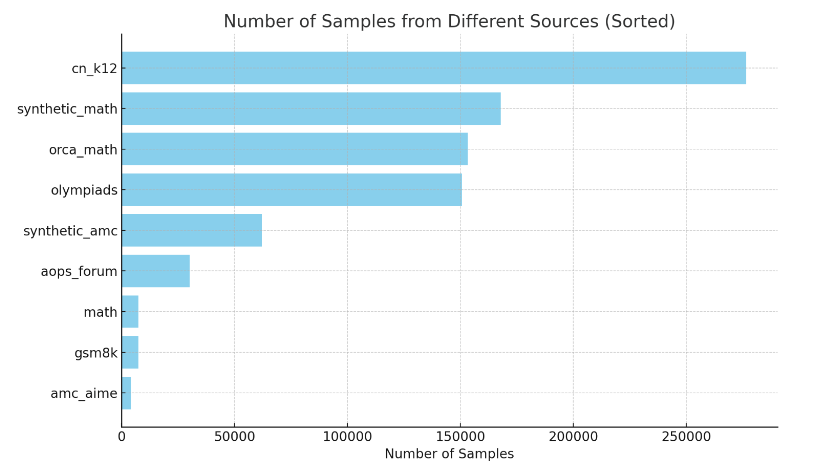
\includegraphics[scale=0.6]{./figures/math_sources.png}
  \caption{Distribution of math sources in the NuminaMath-CoT dataset.}
  \label{fig:math-sources}
\end{figure}

It is important to note that there is an imbalance of problems in the dataset. The most frequent math topics, such as algebra and geometry, are disproportionately more represented than the remaining categories.

\subsection{Data Formatting}

Problems and solutions are formatted using LATEX. The usage of LATEX ensures that the data is easily readable and is easy to parse and process for training the model.

The data for the MATH Dataset is formatted as a JSON file, with each problem containing the following fields:
\begin{itemize}
  \item problem: The text of the problem
  \item level: The difficulty level of the problem (Level 1 up to Level 5)
  \item type: The type of math problem (e.g. Number Theory, Geometry, Algebra, Prealgebra, Counting \& Probability, Precalculus, Intermediate Algebra)
  \item solution: The solution to the problem
\end{itemize}

The data for the Numina Math CoT dataset are formatted as a JSON file, with each problem containing the following fields:
\begin{itemize}
  \item An array of objects, where the first object contains
      \begin{itemize}
        \item content: The text of the problem
        \item role: the role assigned to the person who can access this data (user)
      \end{itemize}
  \item The second object contains
      \begin{itemize}
        \item content: The solution to the problem
        \item role: the role assigned to the person who can access this data (assistant)
      \end{itemize}
\end{itemize}

\subsection{Data Preprocessing}

We converted the data into the following format:
\begin{itemize}
  \item problem: The text of the problem
  \item solution: The solution to the problem
\end{itemize}

In this way, the features and labels are clearly defined, making it easier to train the model. 

Then, we filtered all foreign characters and symbols (i.e. Chinese characters) from the data to ensure that the model is trained on clean and consistent data. This preprocessing step helps to remove any noise or irrelevant information that could affect the model's performance.

Finally, we tokenized the text data using the MathBERT tokenizer, which is specifically designed for mathematical tasks. This tokenizer splits the input into subword tokens that represent both natural language components and mathematical symbols, enabling the model to process math-related queries effectively.

\subsection{Data Splitting}
We split the data into training, validation, and test sets. The training set is used to train the model, the validation set is used to tune hyperparameters and prevent overfitting, and the test set is used to evaluate the model's performance on unseen data.

The split is as follows:
\begin{itemize}
  \item Training set: 80\%
  \item Validation set: 10\%
  \item Test set: 10\%
\end{itemize}

We distributed the Numina CoT dataset across the training, validation, and test sets. However, since the MATH dataset only had 12.5k problems, it was merged with the test set to evaluate the model's performance on a different set of problems.

\section{Model Architecture}

The model architecture is based on the T5 Transformer framework utilizing mathBERTs tokenizer and embeddings, designed to process and generate sequences efficiently. This model leverages a modular design consisting of an encoder-decoder structure tailored for natural language understanding and generation tasks. The architecture is parameterized to balance computational efficiency and performance, making it adaptable to various downstream applications.

\subsection{Encoder}

The encoder is responsible for processing the input sequence and encoding it into a high-dimensional representation that captures its semantic and syntactic structure. It consists of a stack of $N$ identical layers, where each layer has the following components:
\begin{itemize}
    \item \textbf{Multi-Head Self-Attention:} Captures dependencies across all positions in the input sequence, allowing the model to focus on relevant tokens regardless of their distance. The scaled dot-product attention mechanism is computed as:
    \[
    \text{Attention}(Q, K, V) = \text{softmax}\left(\frac{QK^\top}{\sqrt{d_k}}\right)V,
    \]
    where $Q$, $K$, and $V$ represent the query, key, and value matrices, respectively.
    \item \textbf{Feed-Forward Network (FFN):} Applies two linear transformations separated by a ReLU activation, enabling non-linear feature learning. The FFN is parameterized as:
    \[
    \text{FFN}(x) = \text{ReLU}(xW_1 + b_1)W_2 + b_2.
    \]
    \item \textbf{Layer Normalization and Residual Connections:} Layer normalization ensures numerical stability, while residual connections facilitate gradient flow during training.
\end{itemize}

Each layer in the encoder outputs a contextualized representation for every token in the input sequence.

\subsection{Decoder}

The decoder generates the target sequence one token at a time, conditioned on both the encoder outputs and the previously generated tokens. Similar to the encoder, it consists of $M$ identical layers with additional mechanisms to incorporate encoder information:
\begin{itemize}
    \item \textbf{Masked Multi-Head Self-Attention:} Ensures that predictions at position $t$ depend only on tokens up to $t-1$ by masking future positions in the attention computation.
    \item \textbf{Cross-Attention:} Attends to the encoder's outputs to integrate contextual information from the input sequence. The attention mechanism operates on the encoder's key-value pairs and the decoder's queries.
    \item \textbf{Feed-Forward Network:} Identical to the encoder's FFN, applied to each decoder layer.
\end{itemize}

The decoder outputs logits for the target vocabulary, which are transformed into probabilities using a softmax layer.

\subsection{Positional Encoding}

Since transformers lack an inherent notion of sequence order, positional encodings are added to the token embeddings to incorporate positional information. The positional encoding vector is defined as:
\[
PE_{(pos, 2i)} = \sin\left(\frac{pos}{10000^{2i/d_{\text{model}}}}\right), \quad PE_{(pos, 2i+1)} = \cos\left(\frac{pos}{10000^{2i/d_{\text{model}}}}\right),
\]
where $pos$ is the position and $i$ is the dimension index.

\subsection{Training Objective}

The model is trained using a cross-entropy loss function, defined as:
\[
\mathcal{L} = -\sum_{t=1}^T y_t \log p(y_t|y_{<t}, x),
\]
where $y_t$ is the target token at time $t$, and $p(y_t|y_{<t}, x)$ is the predicted probability of $y_t$ given the input sequence $x$ and previously generated tokens.

\subsection{Parameterization}

The model's configuration includes:
\begin{itemize}
    \item \textbf{Hidden Dimension ($d_{\text{model}}$):} 768.
    \item \textbf{Number of Attention Heads:} 8.
    \item \textbf{Feed-Forward Dimension ($d_{\text{ff}}$):} 2048.
    \item \textbf{Number of Encoder Layers:} 6.
    \item \textbf{Number of Decoder Layers:} 6.
    \item \textbf{Dropout Rate:} 0.1.
\end{itemize}

This configuration results in a model with approximately 220 million parameters.

% \subsection{Implementation Details}

% The model is implemented in PyTorch, leveraging Hugging Face's Trainer API for training. It supports mixed-precision training and is optimized using AdamW with a learning rate schedule.



% The proposed model aims to combine the strengths of symbolic math-solving with neural language understanding by utilizing a hybrid architecture that integrates \texttt{LaTeX2SymPy} for parsing mathematical expressions, the \texttt{mathBERT} tokenizer and encoder for understanding the natural language problem, \texttt{SymPy} for symbolic manipulation and computation, and a Seq2Seq decoder for generating textual output. The architecture is designed to be lightweight, efficient, and open-source, making it accessible for deployment in a wide range of applications.

% \subsection{Input Layer: LaTeX2SymPy Parsing}

% The input to the model is a natural language mathematical problem, often expressed in LaTeX format. To handle the structured mathematical expressions present in LaTeX format, we use \texttt{LaTeX2SymPy}. This component parses the LaTeX input into a symbolic expression that can be processed by the subsequent layers.

% \begin{itemize}
%     \item \textbf{LaTeX Parsing:} Convert LaTeX-based input strings into tokenized symbolic expressions.
%     \item \textbf{Symbolic Representation:} Map the parsed LaTeX expressions into \texttt{SymPy} objects, which represent mathematical terms, operators, and functions in a format suitable for algebraic manipulation.
% \end{itemize}

% This parsing step ensures that the mathematical problem is represented in a structured and mathematically accurate form, making it ready for further symbolic operations.

% \subsection{SymPy Solver}

% Once the problem is tokenized and embedded by the MathBERT encoder, it is passed to the \texttt{SymPy} Solver for symbolic computation. \texttt{SymPy} is a Python library dedicated to symbolic mathematics, and its role in this architecture is twofold:

% \begin{itemize}
%     \item \textbf{Symbolic Manipulation:} \texttt{SymPy} is used to perform algebraic simplifications, differentiation, integration, solving equations, and other symbolic manipulations based on the parsed mathematical expression. This step leverages the full symbolic capabilities of \texttt{SymPy} to compute exact solutions when possible.
%     \item \textbf{Mathematical Inference:} For problems requiring a numerical solution (such as solving equations), \texttt{SymPy} can use numerical solvers to provide an approximate answer. \texttt{SymPy} supports a wide range of operations, ensuring that the model can handle complex algebraic, calculus, and number-theoretic problems.
%     \item \textbf{Generation of Subexpressions} The SymPy solver processes a given function one step at a time. To simulate the process of arriving at a mathematical solution, we feed the given expression into SymPy, then repeatedly feed the output expression into the SymPy until a solution is arrived. The generated subexpressions are sequentially concatenated in the order that they are produced, and the final string is passed into the tokenizer. The goal is for the model to not only learn the positional embeddings and the underlying relations behind the word and mathematical expression parts of a given problem, but also to learn the explicit steps leading up to the solution. 
% \end{itemize}

% This integration ensures that the model not only understands the mathematical structure of the problem but also can derive precise and reliable solutions when applicable.

\subsection{MathBERT Tokenizer and Encoder}

The parsed mathematical expression is fed into a \texttt{MathBERT} tokenizer and encoder, which is a specialized version of BERT fine-tuned for mathematical tasks \cite{mathBERT}. MathBERT has been trained to handle both natural language and symbolic mathematical notation, which allows it to effectively process math-related queries and understand the underlying structure of the problem. The steps involved are as follows:

\begin{itemize}
    \item \textbf{Tokenization:} The \texttt{MathBERT} tokenizer splits the input into subword tokens that represent both natural language components and mathematical symbols. This step is crucial for handling mixed inputs such as text-based questions and mathematical formulas.
    \item \textbf{Contextual Embedding:} The tokenized input is passed through the \texttt{MathBERT} encoder, which generates contextual embeddings for each token. These embeddings capture semantic relationships between mathematical operations, variables, and their corresponding natural language descriptions. The encoder's attention mechanism enables the model to focus on relevant parts of the input when generating solutions.
\end{itemize}

% \subsection{Seq2Seq Decoder}

% The final step of the architecture involves the use of a Seq2Seq decoder, which generates the natural language output from the symbolic solution obtained from \texttt{SymPy}. The decoder is designed to convert symbolic results back into human-readable text, making the solution interpretable and usable for end-users.

% \begin{itemize}
%     \item \textbf{Input:} The output from \texttt{SymPy} (whether symbolic or numeric) is used as input to the decoder.
%     \item \textbf{Generation:} The Seq2Seq model is trained to map the symbolic solution into a sequence of natural language words or sentences. This component ensures that the model can output the solution in an understandable and grammatically correct format.
% \end{itemize}

This step integrates both symbolic manipulation and natural language generation, ensuring that the solution is not only mathematically accurate but also linguistically appropriate.

\newpage

\section{Model architecture figure}
% A figure that helps show the overall model or idea. The
% idea is to make your paper more accessible, especially
% to readers who are starting by skimming your paper.
% You must create a new figure, not just use someone
% else's, even with attribution. Be careful that all figure
% text are legible, and are approximately the same size
% as the main text.

Below is a simplified overview of the model architecture, which consists of a tokenization step, an embedding layer, an encoder, a decoder, and an output layer. The tokenization step converts the input sequence into tokens, which are then embedded into a dense vector space. The encoder processes the embedded tokens to extract contextual representations, while the decoder generates the output sequence based on the encoder's outputs. The final output is a sequence of tokens that represent the solution to the input problem.

\begin{figure}[htbp]
  \centering
  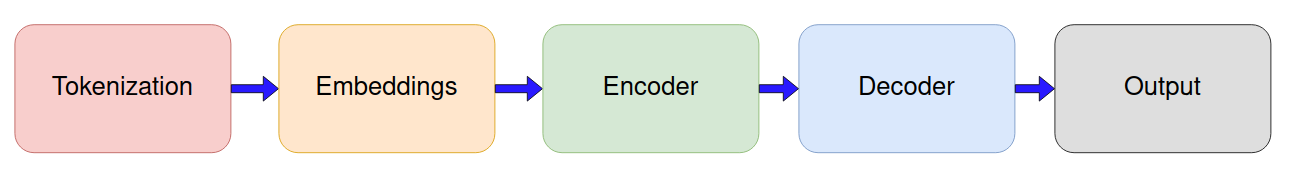
\includegraphics[width=\textwidth]{./figures/model_simplified.png}
  \caption{The Transformer - model architecture.}
  \label{fig:model-arch}
\end{figure}

We will describe each component in detail in the following sections.

\begin{figure}[htbp]
  \centering
  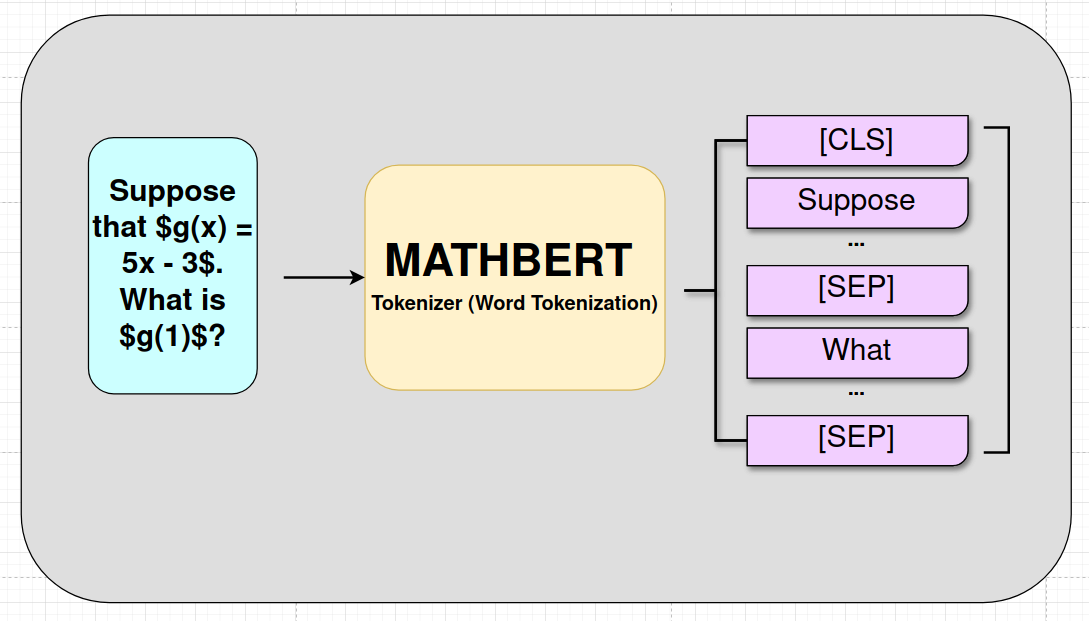
\includegraphics[width=0.7\textwidth]{./figures/tokenization.png}
  \caption{Tokenization of the input sequence.}
  \label{fig:tokenization}
\end{figure}

Tokenization is the process of converting raw text into smaller units, or tokens, that the model can process. In our architecture, we employ subword tokenization to handle diverse vocabulary efficiently, breaking words into meaningful subunits while retaining their contextual integrity. This ensures that the model can effectively encode both natural language and symbolic mathematical expressions, providing a seamless input representation for downstream processing.

\begin{figure}[htbp]
  \centering
  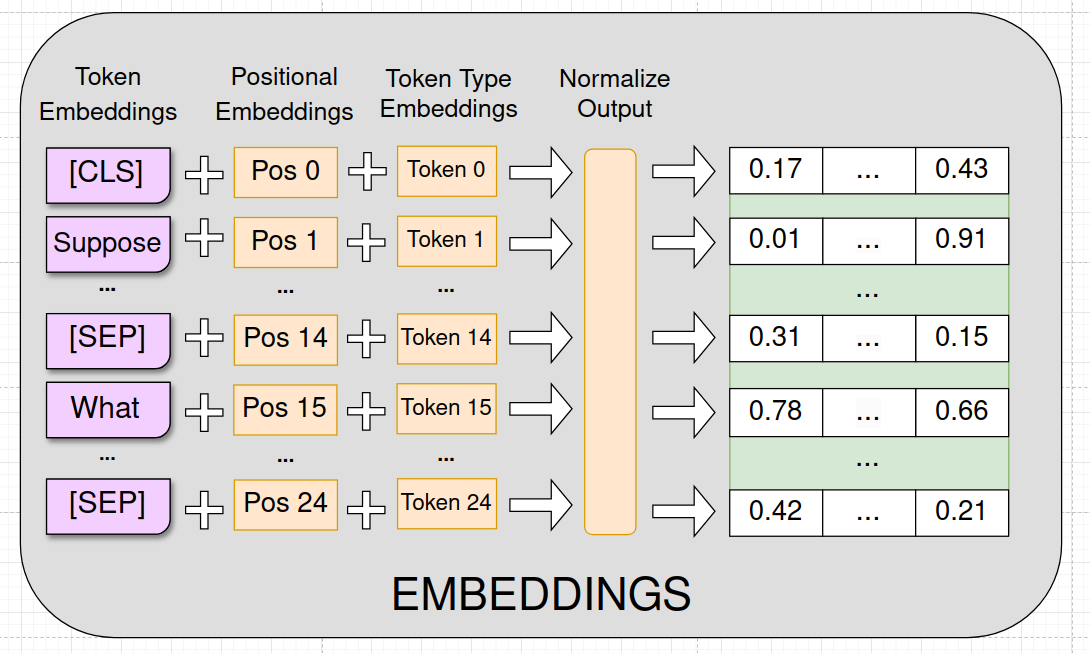
\includegraphics[width=0.6\textwidth]{./figures/embeddings.png}
  \caption{Embedding layer mapping tokens to dense vectors.}
  \label{fig:embeddings}
\end{figure}

Embeddings are dense vector representations of tokens that capture their semantic and contextual meaning. In our architecture, each token is mapped to a fixed-dimensional embedding space, enabling the model to understand relationships between words and symbols. These embeddings serve as the foundation for processing input sequences, preserving both linguistic and mathematical nuances for effective problem-solving.

\begin{figure}[htbp]
  \centering
  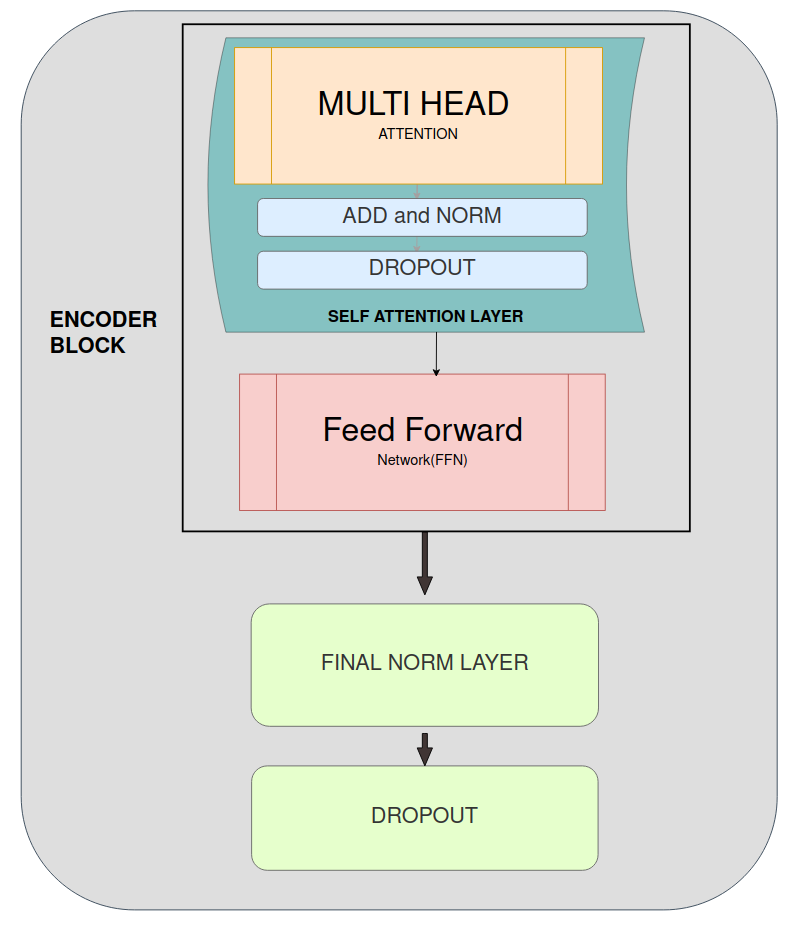
\includegraphics[width=0.5\textwidth]{./figures/encoder.png}
  \caption{Encoder processing the embedded input sequence.}
  \label{fig:encoder}
\end{figure}

The encoder is the core component of our architecture that processes input embeddings to extract contextual representations. It uses self-attention mechanisms to capture relationships between tokens across the entire sequence, ensuring a deep understanding of both natural language and mathematical structures. This allows the model to generate rich, context-aware representations essential for solving complex problems.

\begin{figure}[htbp]
  \centering
  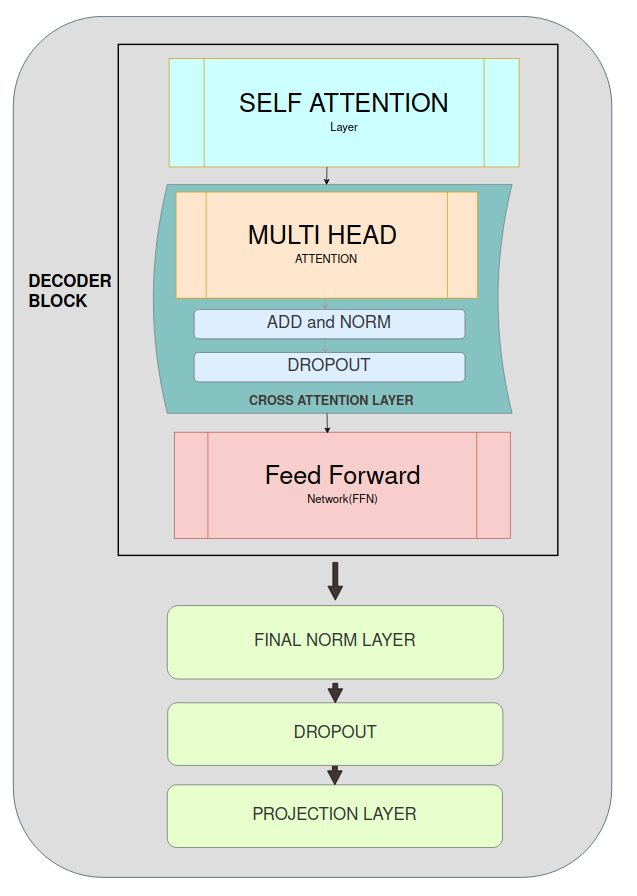
\includegraphics[width=0.4\textwidth]{./figures/decoder.png}
  \caption{Decoder generating the output sequence.}
  \label{fig:decoder}
\end{figure}

The decoder transforms contextual representations from the encoder into meaningful outputs, It consists of 6 stacked decoder blocks, each processing the output from the previous block. Each block includes a self-attention layer to capture relationships within the target sequence, a cross-attention layer to focus on relevant encoder outputs, and a feed-forward layer (FFN) for further refinement. After each layer, add \& norm and dropout are applied for stability and regularization.

\begin{figure}[htbp]
  \centering
  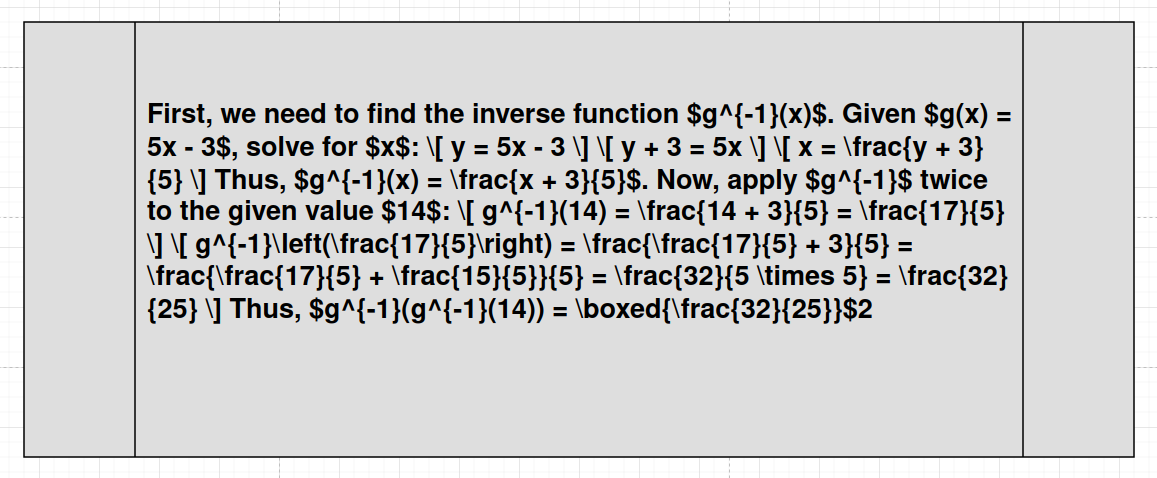
\includegraphics[width=0.7\textwidth]{./figures/output.png}
  \caption{Final output generated by the model.}
  \label{fig:output}
\end{figure}

The final output generated by the model represents the solution to the input problem. The output is a sequence of tokens that can be converted back into human-readable text or LaTeX format, providing a clear and interpretable solution for the given mathematical problem.


\section{Results}
% Describe the performance of your model, either
% quantitatively or (for generative models) qualitatively. To
% help interpret the model, compare your model with a
% baseline model. Qualitative evaluation is OK.


\section{Discussion}
% Interpret the results of your model. If appropriate,
% compare the model performance with the baseline.
% Discuss other features that you notice about the model.


\section{Limitations}
% Describe some settings in which we’d expect your
% approach to perform poorly, or where all existing
% models fail. Try to guess or explain why these
% limitations are the way they are. Give some examples
% of possible extensions, ways to address these
% limitations or open problems

% The limitations section is where you point out the failure cases of the model and highlight where future work must be done

One limitation is related to the embeddings used in our model. We utilized MathBert embeddings, which were pretrained on natural language processing (NLP) tasks for mathematical understanding, such as summarization, detecting mathematical formulas, and auto-grading of student performance. However, these embeddings are not specifically designed for mathematical reasoning, which is crucial for our model's purpose. As a result, our model significantly relies on the fine-tuning of the T5 Encoder-Decoder. Given the limited resources, the fine-tuning process may not have been sufficient to fully adapt the embeddings for strong mathematical reasoning, and additional training could potentially improve the model's performance. Future work could also explore integrating symbolic semantic analysis to enhance the model's understanding and handling of complex mathematical problems. \cite{mathBERT}

Furthermore, the model consists of mainly algebraic problems, which may limit its performance on other types of mathematical problems, such as geometry, calculus, or number theory. The lack of diversity in the training data could cause the model to overfit to the training set, leading to biases in the model's predictions and hinder its generalizability to a broader range of mathematical tasks. To address this limitation, future work could focus on expanding the dataset to include a more diverse set of mathematical problems, ensuring that the model is robust and effective across various domains.

Lastly, the final limitation of our model is the restricted computing resources, as it was trained on a Google Colab Tesla T4 GPU. In comparison, popular large language models such as ChatGPT, Claude, and Bard were trained for significantly longer periods on much larger datasets and with more extensive computational resources. This disparity in training time and resources means that our model could potentially perform better if it were trained with more computational power. Additionally, the lack of parallelization in our training process further limits the efficiency and scalability of our model. Implementing parallelization techniques could significantly reduce training time and improve model performance by leveraging multiple GPUs or distributed computing resources.


\section{Ethical considerations}
% Potential ethical issues posed by the use or misuse of
% your model. Your report should transparently
% communicate the known or anticipated consequences
% of building and using machine learning models on this
% task.

% https://neurips.cc/public/EthicsGuidelines


One ethical consideration is the use of the model in competitive or professional settings, where reliance on the model could lead to unfair advantages or undermine the credibility of the work produced. In competitive exams or professional certifications, using the model to generate solutions could be considered unethical and devalue the merit of the qualifications, while in professional settings, using the model without proper understanding could result in subpar work quality and potential professional misconduct. To mitigate the risk of misuse, clear guidelines and policies should be established regarding the appropriate use of the model, such as prohibiting its use in exams or certifications and implementing measures to detect and prevent cheating. In professional environments, the model should serve as a supplementary tool to assist with tasks rather than replace grading or evaluation, ensuring that the model's use is aligned with ethical standards and minimizing the risk of misuse.

Another ethical issue is the potential for dataset-related biases, as the training data predominantly consists of problems from US contests and Chinese school exercises, which may lead to the model performing better on those types of problems while underperforming on problems from other regions or educational systems. Additionally, the dataset mainly consists of algebra-related questions, which could result in unequal performance and biased grading, as the model may not be equally effective across all types of problems. To mitigate this risk, the dataset should be expanded to ensure diversity and representation from a wide range of problems across different regions, educational systems, and difficulty levels. This can be achieved by curating a balanced dataset from various sources, while regularly evaluating the model's performance to identify and address any biases.

Finally, the last ethical issue is intellectual property rights, as the model is trained on copyrighted data, which could inadvertently promote plagiarism if it provides solutions that students submit as their own, undermining the learning process and leading to academic dishonesty. In professional settings, using the model to generate solutions without proper attribution could violate intellectual property rights and ethical standards. To mitigate this risk, it is essential to ensure that the data used to train the model is properly licensed and that the model does not directly reproduce copyrighted material. This can be achieved by using open-source datasets or those with appropriate licenses for educational use, and by adding a disclaimer to the model's output to indicate that the solution is generated by the model and should be verified and properly attributed before use. Promoting ethical use and proper attribution can help minimize the risk of intellectual property rights violations.


% NOT TO BE INCLUDED IN THE FINAL REPORT
% \section{Work division}
% #TODO: change work division to be that of the actual project
% A description of how the work will be divided between
% the team members, and how the team members will be
% working together (e.g. meet every week Tuesday 4-5
% pm).

% \section*{Writing Components}
% The work will be split as follows:
% \begin{itemize}
%   \item \textbf{Chloe} - Background and Related Work, Abstract, Model Architecture, Results
%   \item \textbf{Takia} - Model Architecture Figure, Model Architecture, Discussions
%   \item \textbf{Gabriel} - Introduction, Model Architecture, Conclusion
%   \item \textbf{Taha} - Data, Ethical Considerations, Model Architecture, Limitatations
% \end{itemize}

% The team will work on each part and meet every weekend for additional discussions.

% \section*{Technical Section}

% \subsection*{Data-Related Tasks (Taha)}
% \begin{itemize}
%   \item Collecting and cleaning large datasets.
%   \item Tokenizing text data.
%   \item Creating and managing training, validation, and test datasets.
% \end{itemize}

% \subsection*{Model Architecture and Development Tasks (Chloe)}
% \begin{itemize}
%   \item Designing the encoder and decoder architecture.
%   \item Implementing the transformer model (attention mechanisms, multi-head attention, etc.).
%   \item Ensuring model components (BERT, etc.) work seamlessly together.
% \end{itemize}

% \subsection*{Training and Optimization (Gabriel)}
% \textbf{Responsibilities:}
% \begin{itemize}
%   \item Setting up the training pipeline.
%   \item Hyperparameter tuning (learning rate, batch size, etc.).
%   \item Implementing and testing various optimization techniques (Adam, gradient clipping, learning rate schedules).
% \end{itemize}

% \subsection*{Evaluation and Visualizations (Takia)}
% \textbf{Responsibilities:}
% \begin{itemize}
%   \item Evaluating model performance using appropriate metrics (BLEU score, perplexity).
%   \item Developing visualization tools to monitor training and validation performance.
%   \item Deciding what metrics to measure the model on.
% \end{itemize}



\section{Conclusion}

% A description of how the work will be divided between
% the team members, and how the team members will be
% working together (e.g. meet every week Tuesday 4-5
% pm).

\bibliographystyle{unsrt}
\bibliography{references}

\end{document}